\documentclass[conference]{IEEEtran}
\IEEEoverridecommandlockouts
% The preceding line is only needed to identify funding in the first footnote. If that is unneeded, please comment it out.
%Template version as of 6/27/2024
\usepackage{booktabs}
\usepackage{array}
\usepackage{geometry}
\geometry{a4paper, margin=1in}
\usepackage{cite}
\usepackage{amsmath,amssymb,amsfonts}
\usepackage{algorithmic}
\usepackage{graphicx}
\usepackage{textcomp}
\usepackage{xcolor}
\def\BibTeX{{\rm B\kern-.05em{\sc i\kern-.025em b}\kern-.08em
    T\kern-.1667em\lower.7ex\hbox{E}\kern-.125emX}}
\begin{document}

\title{Bayesian Modelling and Prediction of High Drug Intake  in Bangladesh\\
% {\footnotesize \textsuperscript{*}Note: Sub-titles are not captured for https://ieeexplore.ieee.org  and
% should not be used}
% \thanks{Identify applicable funding agency here. If none, delete this.}
}

\author{\IEEEauthorblockN{Syeda Rija Hasan Abidi}
\IEEEauthorblockA{\textit{Computer Science} \\
\textit{Habib University}\\
Karachi, Pakistan \\
sa07424@st.habib.edu.pk}
\and
\IEEEauthorblockN{Muminah Khurram}
\IEEEauthorblockA{\textit{Computer Science} \\
\textit{Habib University}\\
Karachi, Pakistan \\
mk07521@st.habib.edu.pk}
\and
\IEEEauthorblockN{Raza Hashim Nizamani}
\IEEEauthorblockA{\textit{Computer Science} \\
\textit{Habib University}\\
Karachi, Pakistan \\
rn07380@st.habib.edu.pk}
}

\maketitle

\begin{abstract}
This project develops a Bayesian network model to predict susceptibility to drug addiction in Bangladesh, focusing on demographical, psychological, and socio-economic factors such as age, gender, living conditions, mental health, stress, and education. By analyzing these variables with input from domain experts and various data sources, the model will assist stakeholders such as psychologists and counselors in identifying individuals at higher risk for addiction, facilitating early intervention, and informed support strategies in rehabilitation while also highlighting the addiction susceptibility of a wide range of individuals paving the way for policymakers to combat this rising problem on a large scale.\end{abstract}

\begin{IEEEkeywords}
Bayesian Network, Addiction, Bangladesh, Machine Learning, Structure Learning.
\end{IEEEkeywords}

\section{Introduction}
% Drug abuse and addiction have been identified as a major problem in Pakistan by the World Health Organization (WHO) \cite{emhj_drug_users_karachi} with 4.25 million drug users identified in 2023 and the number is only growing \cite{unodc_survey_drug_use_pakistan}. With societal neglect, lack of resources for rehabilitation facilities, and non-existent regulation by authorities, this problem is worsening by the year. Generally, the risk of addiction goes unheeded with few tools for practitioners at rehabs such as psychologists and counselors to deduce the susceptibility based on the symptoms and demographics of the patient. 

% In this project, we will model the susceptibility of individuals to develop drug dependence and addiction, given a multitude of factors such as age bracket, gender, living conditions, psychological health, stress levels, education, etc. in the context of Bangladesh. We aim to create a Bayesian network with causes and effects of addiction defined with the help of datasets and domain experts. 
Drug abuse and addiction have been identified as a major problem in Bangladesh by the Department of Narcotics Control (DNC) and other national bodies, with estimates suggesting there are over 3.6 million drug users in the country as of 2018 \cite{unodc_news_2024}. Young men, aged 15 to 30 make up around 85\% of consumers but a recent consumption rise has been observed in women \cite{pmc8554893}. This rise is indicative of a growing public health crisis that continues to worsen due to societal neglect, lack of resources for rehabilitation facilities, and insufficient regulatory oversight by authorities that could be responsible for the disruption of family dynamics, escalated social isolation, imposition of economic burdens and contribute to criminal activity \cite{emerald_drug_crisis_2024}.
The problem is exacerbated by the limited availability of tools and resources for psychologists, counselors, and practitioners working in rehabilitation facilities. Many practitioners lack effective methodologies to deduce the susceptibility of individuals to addiction based on their symptoms and demographic profiles \cite{PMC8294555}. This gap hampers early intervention and tailored treatment approaches, further compounding the crisis. In this project, we aim to model the susceptibility of individuals to develop drug dependence and addiction, given a multitude of factors such as age bracket, gender, living conditions, psychological health, stress levels, education, etc. in the context of Bangladesh. We aim to create a Bayesian network with causes and effects of addiction defined with the help of datasets and domain experts that can serve as a diagnostic tool for drug addiction. 


\section{Literature Review}
Using probabilistic reasoning through Bayesian networks to detect addiction patterns has many different forms in the literature. Gnanasekar et al. use a Bayesian network and image classification to create a causal model to predict drug addicts based on drug abuse marks on their faces and “soft” face biometrics. This amalgamation of neural networks with Bayesian networks yielded 84\% accuracy. The root node here is “Drug Abuser” and its effect attributes (directed arrow to) are the nodes of Blisters/Acne, Muscle loss, Hair loss, Poor Skin tone, and Gender. The study uses a diagnostic or bottom-up approach where they infer from the images whether the person is an addict or not \cite{gnanasekar_face_attributes_drug_addicts}. Our project takes a complementary approach to Gnanasekar et al.’s study; while their study uses symptoms of drug addiction to determine whether an individual is currently struggling with addiction, our focus is on predicting the likelihood of future addiction based on various sociodemographic and psychological factors.

Another study targeting addiction using Bayesian Networks was on Internet Addiction Disorder (IAD) \cite{singh_internet_addiction_bayesian}. This study established causal links between Internet Addiction and what might be observed as symptoms, we aim to achieve something similar with our study. Doing so would make it easier for stakeholders to identify addiction using all its different manifestations and also identify its severity. Their model made erroneous predictions 5.7\% of the time, showcasing the potential of applying Bayesian Networks to a problem very similar to ours. The causal links also aid in establishing a sense of prioritization as to what the most relevant factors are and where the efforts should be focused. The study models 5 causal attributes while one effect attribute — the presence of IAD. Both predictive and diagnostic reasoning are shown with evidence of the causal and effect attributes. While the primary aim of our study is to predict the susceptibility of individuals to addiction, we can also perform diagnostic reasoning i.e. with the presence of addiction we may deduce the likelihood of their demographics, socio-economic situation, and so on.

A major study that works on the same problem statement as this project is that of Abada et al. where they constructed a Naïve Bayes classification model to predict the likelihood of drug addiction. The parameters considered in the model were demographics, socioeconomic status, proximity to drugs, conflict with law, failure in life, and psychological attributes. This data consists of 26 total attributes and 205 instances. This study yields an accuracy score of 91\% indicated by the evaluation metrics of High Detection Rate, False Alarm, Accuracy, Precision, and F-measure \cite{abada_bayesian_model_drug_addiction}. While we will be working with the same attributes as Abada et al., we will not be considering the attributes to be independent as done in this Naïve Bayes model. However, the evaluation metrics to gauge the accuracy will remain the same.

Contextually, recent studies have explored the multifaceted issues surrounding drug addiction in Bangladesh, especially in light of the heightening tensions following the country's crackdown on drugs in 2018. Islam highlights the importance of socioeconomic disparities, mental health challenges, and social isolation as significant risk factors for drug abuse in the region \cite{drugWarJstor}. They introduce the concept of self-medication as a potential explanatory model, drawing parallels between the coping mechanisms of addicts and non-addicts using painkillers. The analysis further critiques the "war on drugs" approach, illustrating how punitive measures often exacerbate addiction issues by increasing drug prices and incentivizing new entrants into the drug market. These findings emphasize the importance of comprehensive, evidence-based interventions, including harm reduction services, rather than solely relying on enforcement-based policies. This perspective aligns with our focus on leveraging data-driven models like Bayesian Networks to predict and mitigate addiction risks, particularly through a nuanced understanding of contributing factors.

Recent reports provide critical insights into drug addiction trends from the region. Data from the Annual Drug Report Bangladesh conducted in 2022 by their Department of Narcotics Control shows that from 2018 to 2022 a shifting age demographics of drug addiction is seen with a notable increase in patients aged 21-25 (from 19.92\% in 2018 to 20.52\% in 2022) and a corresponding decline among younger age groups like 16-20 years (from 22.51\% in 2018 to 16.76\% in 2022) \cite{dnc2023}. This age shift highlights the evolving risk factors tied to young adulthood, such as socio-economic pressures and increased exposure to illicit substances during formative years. Additionally, statistics on drug seizures reflect the complexity of the illicit drug trade. For instance, the annual confiscation of methamphetamine (Yaba) pills remains alarmingly high, with 53 million seized in 2021 alone \cite{dnc2023}. Meanwhile, the emergence of new synthetic drugs like crystal methamphetamine indicates criminal networks' adaptability to stricter regulatory measures. A map published by the UNODC as part of the World Drug Report highlights significant methamphetamine seizures globally, underscoring South Asia as a critical transit and manufacturing region \cite{unodc2023}. This aligns with existing knowledge on regional drug trade dynamics: Afghanistan's role as a major producer of opiates, along with the porous borders of India and Pakistan, has long facilitated trafficking routes into South Asia, including Bangladesh. The same summary also revealed that opioids remain the primary drug used by people in drug treatment within South Asia. This underscores how the seizures of heroin and cannabis have fluctuated over the years, while newer substances like crystal methamphetamine are increasingly found, suggesting the evolving nature of the illegal drug economy.


% In the context of Pakistan, a cross-sectional survey is provided by Ghazal et al. that investigates the rising trend of drug addiction in Pakistan, focusing on the socio-demographic factors of patients admitted to rehabilitation centers in Islamabad and Rawalpindi. The study found that most addicts were young, skilled individuals, with a significant portion being educated, with heroin being the most abused drug, and peer pressure along with family disputes serving as key drivers of addiction. The study emphasizes the urgent need for preventive measures and highlights the co-morbid presence of depression in nearly half of the 102 participants as well as challenging the traditional notion that drug addiction primarily affects the uneducated and unemployed, showing that addiction is pervasive across various social strata \cite{ghazal_substance_abuse_pakistan}. This paper ends with a call for better rehabilitation facilities and policymaker intervention to address the alarming rise in substance abuse. Following in the footsteps of Ghazal et al. to address this pressing problem, the primary aim of our project is to present a technological and data-driven approach to better equip rehabilitation facilities, practitioners, and policymakers with significant insight into where preventative measures can be targeted by employing sensitivity analyses on our model.



The creation of a Bayesian Network is the key deliverable of this project. This task becomes extremely tedious as the number of variables/nodes under consideration increases. In our project, we will be learning the structure of the Bayesian Network through structure learning to ensure consistency with data and expert advice to introduce context-specific nuances. The task of structure learning, however, is NP-Hard with the number of nodes/variables. Ever since the creation of Bayesian Networks by Judea Pearl in 1985 there have been many approximations and search heuristics techniques developed to combat this computational complexity and approximate the task in a reasonable amount of time. In 2023, Kitson et al. proposed 73 state-of-the-art algorithms and approaches for structure learning \cite{kitson2023survey}. All these approaches can be divided into three main categories: score-based structure learning, constraint-based structure learning, and hybrid models which combine the strengths of score-based and constraint-based structure learning to optimize results \cite{kitson2023survey}. 

The score-based approach is the most common of structure learning approaches and can be more accurate than constraint-based learning depending on the efficacy of the score function used and the size of the data \cite{scanagatta2019survey}. This score function finds the best graph/network from the solution space of all possible graphs based on its fitness to the data. On the other hand, the constraint-based approach utilizes statistical tests to check conditional independencies among variables. These independencies determine the edges in the network. One notable example of this approach is the PC algorithm (named after its authors Peter and Clark) which starts with an undirected complete graph and recursively deletes edges based on independencies \cite{scanagatta2019survey}. The type of approach and algorithm for structure learning heavily depends on the quality, specifications, and size of the data and project requirements. The constraint-based approach is more suited for large datasets as the accuracy of the statistical tests is determined by the sample size while score-based approaches are computationally extremely expensive for large datasets and must be accompanied by heuristic approaches to deal with bigger datasets \cite{scanagatta2019survey}. As we expect to work with a dataset of moderate size, we may harness the power of hybrid models, however, it is subject to change as we are still finding more sources of data. 

As highlighted in this literature review, the feasibility and potential of Bayesian Networks in modeling drug addiction is evident. Yet, relatively few studies have specifically targeted addiction susceptibility prediction—especially in the context of Bangladesh. Existing research on drug addiction factors within Bangladesh, such as the study by Moonajilin et al. catalyzed more attention on the matter and emphasized the urgency of preventative measures for drug addiction, but it was itself qualitative and non-computational \cite{PMC8294555}. Given the rising trend of the problem of drug addiction in Bangladesh, it is high time that this gap in research starts to be filled by technological and data-driven advancements. To this end, our study not only highlights the key factors involved in addiction and their impact but it will also aid stakeholders and practitioners in devising effective mitigating strategies and preemptive measures with the help of Bayesian network modeling. 

\section{Methodology}
\subsection{Dataset}
Our study utilizes a dataset based on Bangladeshi data, containing information on 211 individuals and their drug-using habits \cite{dataset}. This dataset serves as a comprehensive profile of drug users in Bangladesh by taking into account factors such as their age, gender, educational background, financial background, family dynamics, etc. In total, the dataset contained 26 variables that serve as the nodes in the network. However, there exist some inherent biases in the dataset, 89\% of the individuals are under 35, 67\% are male and 63\% are university students,  to address this, we randomized the dataset records using the RAND() function in Excel ensuring an even distribution of all states. It should be noted here that the information shared is self-reported by the individuals themselves as is evident from entries for variables such as "Withdrawal Symptoms". The majority of the variables are non-binary multi-state variables, with some of them having over several unique states, such as the case with 'Mental/emotional problem' having over 16 unique states through combinations of 5 possible options and the variable 'Motive about drug' having over 7 unique states. 

\subsection{Cleaning \& Preprocessing}
For added clarity and coherence within the network, the data was simplified. Firstly we combined the different states of variables with over five unique states into simpler and broader categories. For the "Mental/emotional problem" variable, we broadly categorized data into five distinct states: Depression, Anxiety, Both, Other, and None. Entries containing both Depression and Anxiety were categorized as "Both," while entries with either Depression or Anxiety alone, irrespective of other factors, were categorized as "Depression" or "Anxiety" Finally cases containing neither Depression nor Anxiety were grouped under "None," with any residual combinations falling into the "Other" category. We also simplified the "Finances of Family" variable into income group classes while also merging the "Poor" and "Solvent" categories into a broader "Lower Class" category. Similarly, the "Age" variable was adjusted by combining the 35-48 and above-48 categories into a single "Above 35" group, as there was only one entry in the above-48 category. Ambiguous entries in some variables, such as "I do not know" in the "Withdrawal symptoms" variable, were standardized to "Unsure" to ensure consistency. Additionally, some variable names were revised to improve clarity and reduce ambiguity. For instance, "Enjoyable with" was renamed to "Enjoyable amount of drugs" to reduce ambiguity and ensure a more interpretable dataset. Lastly, the “Motive with drug” node was removed because its seven states, instead of adding meaningful predictive value, introduced excessive variance and noise into the model.

\begin{table}[h!]
\centering
\caption{Standardization Summary}
\label{tab:data_simplification}
\resizebox{\columnwidth}{!}{%
\begin{tabular}{>{\raggedright\arraybackslash}p{3.5cm} >{\raggedright\arraybackslash}p{8cm}}
\toprule
\textbf{Variable}                & \textbf{Simplification / Standardization Description}               \\
\midrule
\textbf{Mental/emotional problem} & Combined into five categories: \textit{Depression}, \textit{Anxiety}, \textit{Both}, \textit{Other}, and \textit{None}. \newline 
Entries with both Depression and Anxiety $\rightarrow$ ``Both''; Depression or Anxiety alone $\rightarrow$ ``Depression'' or ``Anxiety.'' Cases with neither $\rightarrow$ ``None,'' and residual combinations $\rightarrow$ ``Other.'' \\

\textbf{Finances of Family}       & Simplified into income groups. Categories ``Poor'' and ``Solvent'' merged into a broader ``Lower Class.'' \\

\textbf{Age}                      & Combined the ``35-48'' and ``above-48'' categories into a single ``Above 35'' group due to limited entries in the ``above-48'' category. \\

\textbf{Withdrawal symptoms}      & Standardized ambiguous entries like ``I do not know'' to ``Unsure'' for consistency. \\

\textbf{Motive with drug}         & Removed due to excessive variance and noise caused by its seven states, which added minimal predictive value. \\

\textbf{Variable names}           & Revised for clarity and interpretability. \newline 
Example: ``Enjoyable with'' renamed to ``Enjoyable amount of drugs.'' \\

\bottomrule
\end{tabular}%
}
\end{table}
For data entry and preparation for structure and parameter learning, several preprocessing steps were carried out to ensure compatibility with the modeling software. Empty spaces in state names were replaced with underscores, and special characters such as “/” and “.” were removed, as these characters were prevalent in the dataset and could cause issues during processing. Furthermore, state names starting with digits, which are not valid in the modeling framework, were prefixed with an “s” to ensure compliance. For example, “15 to 22 years” was renamed as “s15\_to\_22\_years,” and “H.S.C / A levels” was converted to “HSC\_A\_levels.”

Utilizing the cleaned Bangladeshi dataset, the dataset was split into training and testing subsets, allocating 80\% (169 records) for training and 20\% (42 records) for testing. 

\begin{table}[h!]
\centering
\caption{Cleaning strings for Structure \& Parameter Learning}
\label{tab:preprocessing_steps}
\resizebox{\columnwidth}{!}{%
\begin{tabular}{>{\raggedright\arraybackslash}p{3cm} >{\raggedright\arraybackslash}p{8cm}}
\toprule
\textbf{Step}                      & \textbf{Description} \\
\midrule

\textbf{Empty Spaces Handling}     & Empty spaces in state names were replaced with underscores to ensure compatibility with the modeling software. \\

\textbf{Special Characters Removal} & Special characters such as ``/'' and ``.'' were removed from state names to prevent processing issues. \\

\textbf{State Names Starting with Digits} & State names starting with digits were prefixed with an ``s'' to comply with the modeling framework. \newline 
Example: ``15 to 22 years'' $\rightarrow$ ``s15\_to\_22\_years.'' \\

\textbf{State Name Standardization} & Names containing special characters were adjusted for clarity and consistency. \newline 
Example: ``H.S.C / A levels'' $\rightarrow$ ``HSC\_A\_levels.'' \\

\bottomrule
\end{tabular}%
}
\end{table}

\subsection{Structure \& Parameter Learning}
We learned the structures and parameters of three Bayesian networks using Bayesian Search, Peter and Clark, and Greedy Thick Thinning algorithms. 

Before learning we also forbade non-intuitive edges or links. In initial attempts without any restrictions, nodes like "Education" had edges pointing to "Age" and nodes like Smoking pointing to "Gender." While this could be a valid probability distribution, we forbade anything "causing" Age or Gender. Hence we introduced 49 forbidden links as our prior knowledge as given in Figure 1 and Table III.

\begin{figure}[h]
    \centering
    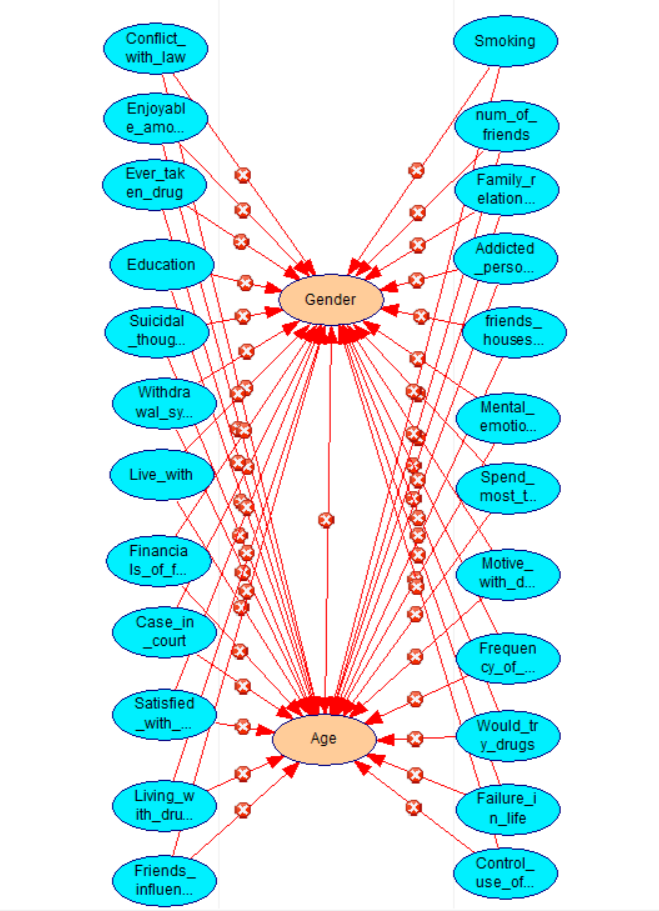
\includegraphics[width=\linewidth]{priorknowledge.png} % Adjust width for fitting
    \caption{Non-intuitive Forbidden Edges}
    \label{fig:forbidden_edges} % Add a label for referencing
\end{figure}


\subsubsection{Bayesian Search Algorithm}
The Bayesian Search Algorithm was originally proposed by Cooper and Herskovitz (1992) and later refined by Heckerman (1995) \cite{genie_structure_learning}. This algorithm follows a hill-climbing procedure guided by a scoring heuristic—in this case, the log-likelihood function as implemented in GENie to ensure that the learned structure captures the most likely relationships among variables. It chooses a starting structure at random, then the log-likelihood function evaluates the structure by calculating how well the model fits the data. Local modifications are performed to the structure by adding, removing, or reversing edges between nodes based on the scoring, to avoid hitting a local maxima, the algorithm periodically restarts from a new random structure. 

\textbf{Parameters for learning:}
The parameters for learning the BN are given in Table III. We tweaked the number of iterations to search for the best network from 50-100 to obtain the most optimal iteration at 100. To reduce complexity and the risk of overfitting, the number of parents was restricted to 4. To evaluate the conditional probabilities, we included 100 samples to make the processing computationally efficient and reduce overfitting. The link probability is set to 0.1 to ensure sparse a graph, which is more interpretable and less prone to overfitting. The prior belief probability is set very low at 0.005 to ensure that edges are only connected if there is a strong statistical correlation.  Finally, the max search time is set to 0 which indicates no time limit, however, the graph still took less than a second because of the small dataset. The node "Frequency of drug use" was set as the target for the network. We aim to check the sensitivity of this node concerning other nodes or factors. In the real world, this maps susceptibility to heightened drug use, which renders individuals incredibly prone to addiction as per our domain expert. Hence, we set the score by the accuracy of predicting the node "Frequency of drug use." The 8-fold cross-validation is used to ensure the prediction is valid. 

\begin{table}[h!]
\centering
\label{tab:learning_summary}
\caption{Bayesian Search Learning Algorithm Parameters}
\renewcommand{\arraystretch}{1.3}
\resizebox{\columnwidth}{!}{%
\begin{tabular}{>{\raggedright\arraybackslash}p{4cm} >{\raggedright\arraybackslash}p{6.5cm}}
\toprule
\textbf{Parameter}                & \textbf{Value / Description}            \\
\midrule
\textbf{Input File}               & finalbanglatrain                        \\
\textbf{Data Rows}                & 169                                     \\
\textbf{Elapsed Time}             & 0.937s                                  \\
\midrule
\textbf{Algorithm Parameters}     & \begin{itemize} 
                                   \item Iterations: 100 
                                   \item Max Parent Count: 4 
                                   \item Sample Size: 50 
                                   \item Link Probability: 0.1 
                                   \item Prior Link Probability: 0.005 
                                   \item Seed: 42 
                                   \item Max Search Time: 0 
                                   \end{itemize} \\
\midrule
\textbf{Score by Accuracy}        & 8-Fold Cross Validation, Class Variable: Frequency\_of\_drugs \\
\textbf{Background Knowledge}     & Forbidden Arcs: 49  \\
\bottomrule


\end{tabular}%
}
\end{table}

\subsubsection{Peter \& Clark Algorithm}
Peter \& Clark (PC) Algorithm is a constraint-based algorithm that identifies conditional independencies between variables to construct a graph. It starts with a fully connected undirected graph where all nodes are connected by edges, edge removal is done between two nodes if they are found to be conditional independent. Once edge removal is complete, the algorithm applies statistical tests to orient the remaining edges, ensuring they maintain conditional independence, acyclicity, and consistency and finally, it outputs a Directed Acyclic Graph (DAG) that reflects the structure of the data.

\textbf{Parameters for learning:}
For the PC algorithm, we considered the whole dataset because it does not have an option for target-based learning. We restricted the same number of maximum in-degree or parents for each node. The p-value or statistical significance was fixed to be 0.01 which ensures that only the strong correlation dependencies are considered.

\begin{table}[h!]
\centering
\caption{Peter \& Clark Algorithm Parameters}
\label{tab:learning_summary}
\renewcommand{\arraystretch}{1.3}
\resizebox{\columnwidth}{!}{%
\begin{tabular}{>{\raggedright\arraybackslash}p{4cm} >{\raggedright\arraybackslash}p{6.5cm}}
\toprule
\textbf{Parameter}                & \textbf{Value / Description}            \\
\midrule
\textbf{Input File}                    & banglafinaltrain                  \\
\textbf{Data Rows}                     & 169                       \\
\textbf{Elapsed Time}                  & 0.078s                    \\
\midrule
\textbf{Algorithm Parameters}          &                           \\
\hspace{1em} Max Adjacency             & 4                         \\
\hspace{1em} Significance              & 0.01                      \\
\hspace{1em} Max Search Time           & 0                         \\
\midrule
\textbf{Background Knowledge}          &                           \\
\hspace{1em} Forbidden Arcs            & 49                        \\
\bottomrule
\end{tabular}%
}
\end{table}

\subsubsection{Greedy Thick-Thinning Algorithm}
The Greedy Thick-Thin algorithm, conceived by Cheng et al., is a Bayesian Search based approach for constructing a Bayesian Network. It also approximates but manages to produce results in a short span of time while yielding good structures. It operates in two phases:
\begin{itemize}
    \item Thick Phase: It starts off with an empty graph and adds edges that maximally increase the marginal likelihood P(D$|$S). It does so in a greedy manner, only considering the local scores.
    \item Thin Phase: After the graph is constructed, it repeatedly removes edges until no edge deletion will result in a positive increase in P(D$|$S). 
\end{itemize}
\textbf{Parameters for learning:}
Like the PC algorithm, the parameters for the Greedy Thick-Thin algorithm are limited. We forbade the same edges and kept the number of parents at 4. Edges pointing to Age and Gender are not considered. 

\begin{table}[h!]
\centering
\caption{Greedy Thick-Thinning Algorithm Parameters}
\label{tab:greedy_tt_results}
\renewcommand{\arraystretch}{1.3}
\resizebox{\columnwidth}{!}{%
\begin{tabular}{>{\raggedright\arraybackslash}p{5.5cm} >{\raggedright\arraybackslash}p{6.5cm}}
\toprule
\textbf{Parameter / Metric}         & \textbf{Value / Description} \\
\midrule
\textbf{Input File}                 & banglafinaltrain                    \\
\textbf{Data Rows}                  & 169                         \\
\textbf{Elapsed Time}               & 0.063s                      \\
\midrule
\textbf{Algorithm Parameters}       & Max Parent Count: 4         \\
\midrule
\textbf{Background Knowledge}       & Forbidden Arcs: 49 \\
\bottomrule
\end{tabular}%
}
\end{table}

\section{Results \& Discussion}
In this section, we will compare all three networks and evaluate the results. We tested all the models for the target node "Frequency of drug use" on the test dataset comprising 42 records. The 5-fold accuracy evaluation was used in all testing. We have performed sensitivity analysis with respect to the ``frequency of drug use'' on each network. The shades of red represent the strength of the influences on the node, the darkest being the strongest and the lightest being the weakest. We have also represented the strength and type of the influences of nodes on their children. The thickness of the edge represents the strength while the color represents whether the influence is positive, negative, or ambiguous. 

\subsection{Bayesian Search Network}
The Bayesian network model was tested on a separate dataset comprising 20\% of the original records, achieving an average accuracy of 70\%. The model reached a maximum accuracy of 75\% at iteration 71. Given the training dataset size of 169 records, this score indicates a reasonable balance between generalization and precision. 

The Expectation-Maximization (EM) log-likelihood was found to be low, as expected since the network was optimized for predicting a single target node rather than all nodes. However, it is still greater than the PC and Greedy ThickThinning networks. This is the most intuitive Bayesian network structure among all three as shown in Figure \ref{fig:BN_model}. 

\begin{figure}[h!]
    \centering
    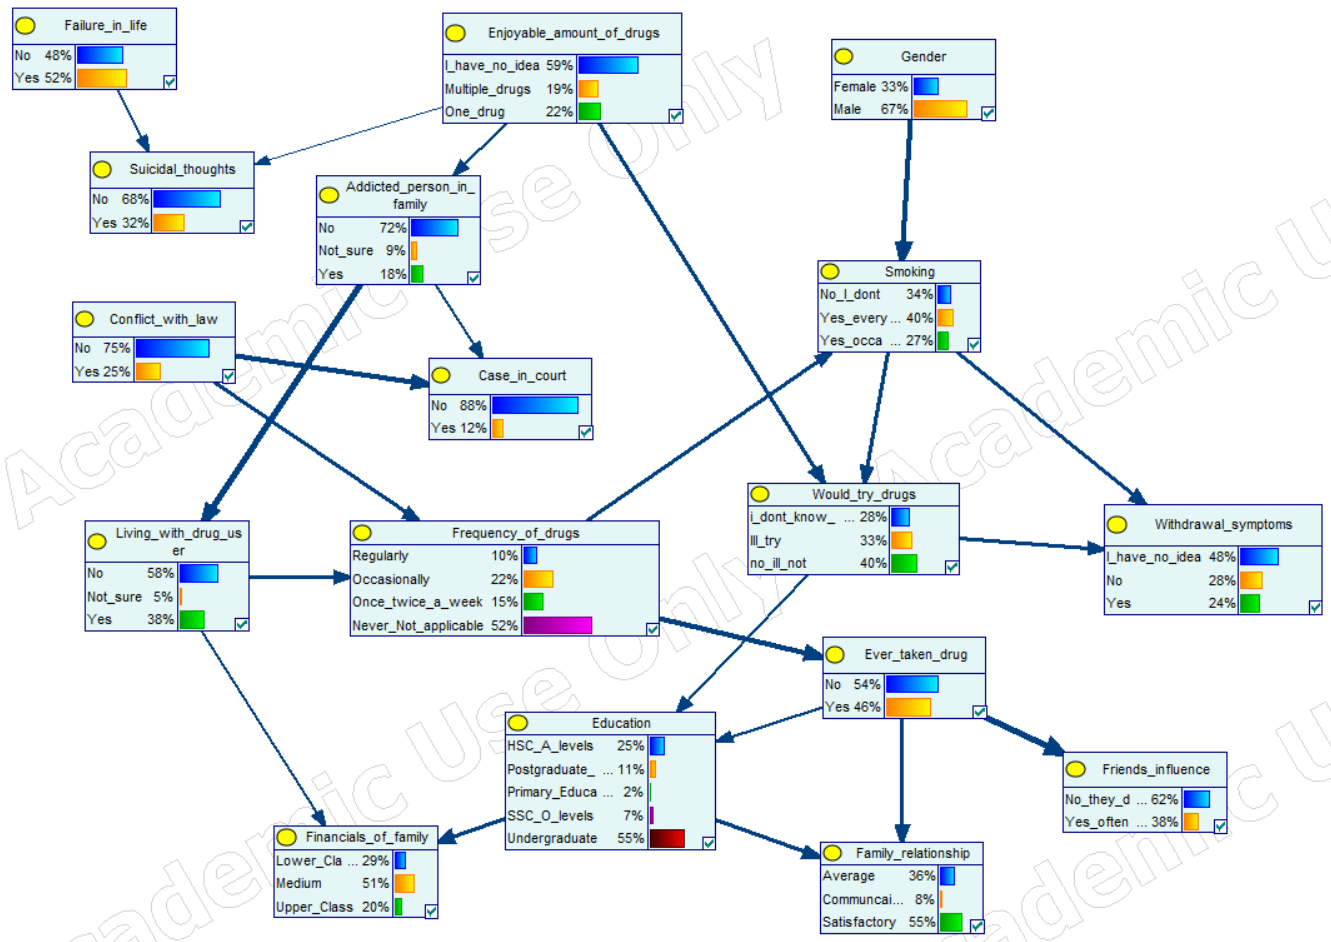
\includegraphics[width=1\linewidth]{BN.png}
    \caption{Bayesian Network for Predicting ``Frequency of Drugs'' Visualized in GeNIe.}
    \label{fig:BN_model}
\end{figure}

\subsubsection{Accuracy}
The predictive accuracy of the Bayesian Search algorithm is shown in Figure \ref{fig:BN_accuracy}. The model demonstrated the peak accuracy of 75\% while training but the testing accuracy was found to be 73.8\%. 

\begin{figure}[h!]
    \centering
    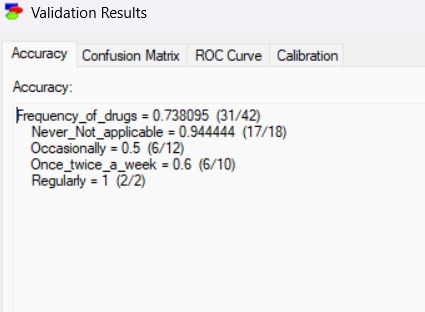
\includegraphics[width=\linewidth]{accuracies/BNSTest.jpg}
    \caption{Bayesian Search Network Accuracy of Prediction.}
    \label{fig:BN_accuracy}
\end{figure}

\subsubsection{Sensitivity Analysis}
The sensitivity analysis on the Bayesian Search network reveals key relationships on the target ``Frequency of Drugs.'' Living with a drug user and conflict with the law have the strongest effect on an individual's frequency of drug use as shown in Figure \ref{fig:sensitivity_BN}

\begin{figure}[h!]
    \centering
    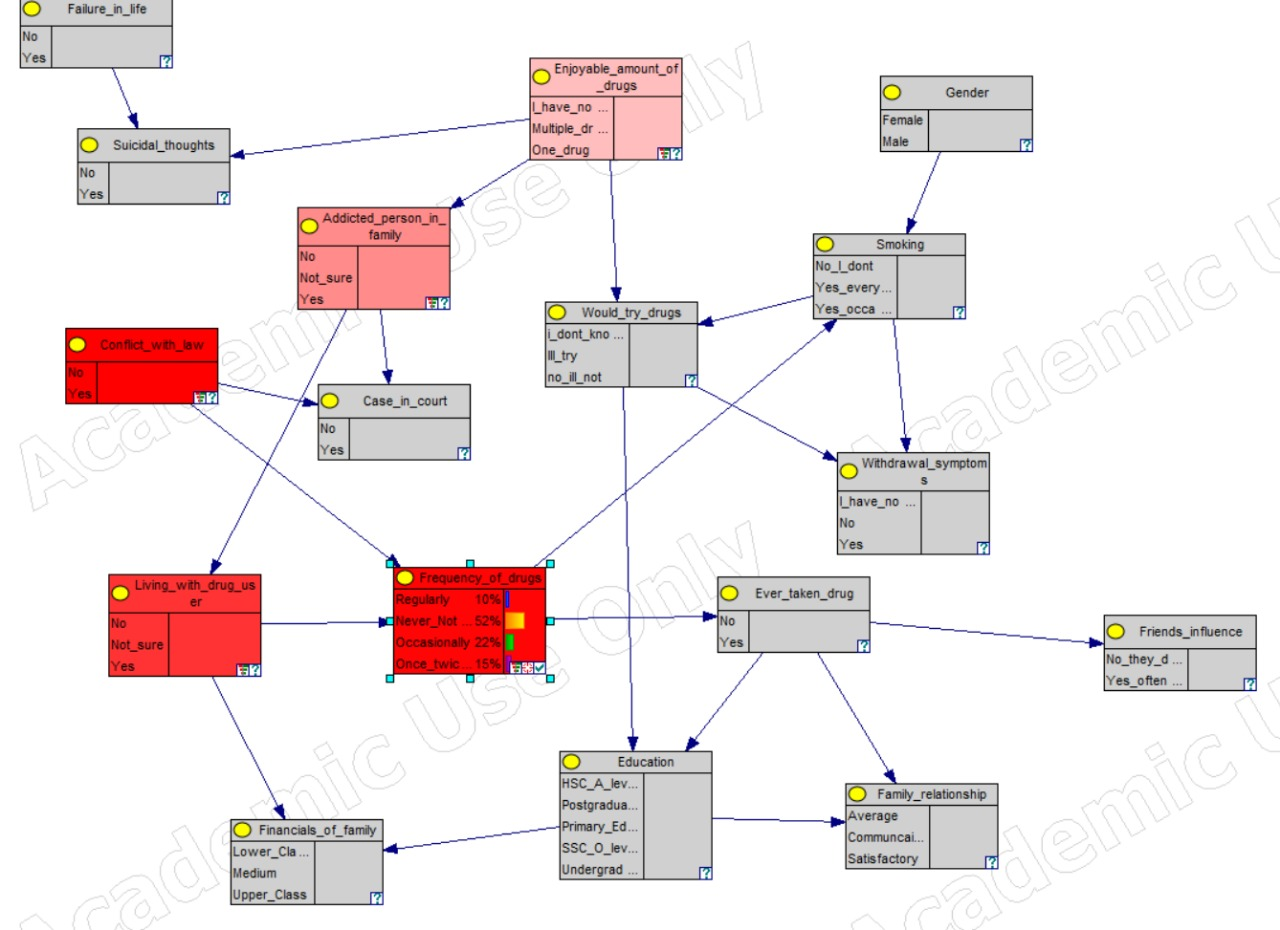
\includegraphics[width=\linewidth]{sensitivity/redBN.jpg}
    \caption{Sensitivity Analysis of Bayesian Network Targeting Drug Frequency.}
    \label{fig:sensitivity_BN}
\end{figure}

\subsubsection{Influence Relations}
The influence diagram shown in Figure \ref{fig:influence_BN} mostly contains purple arrows representing ambiguous relations among nodes. This also means that while one state may have a positive influence child, another state may have an extremely negative influence, adding up to have an overall ambiguous effect. Ever taken drugs negatively influencing family relationships is intuitive because of the negative reaction of one's family towards drug use. The positive influences from failure in life to suicidal thoughts, Gender to smoking, conflict with law to case in court, and ever taken drug to friends' influence are all consistent with the norms and practices of a South Asian society. 


\begin{figure}[h!]
    \centering
    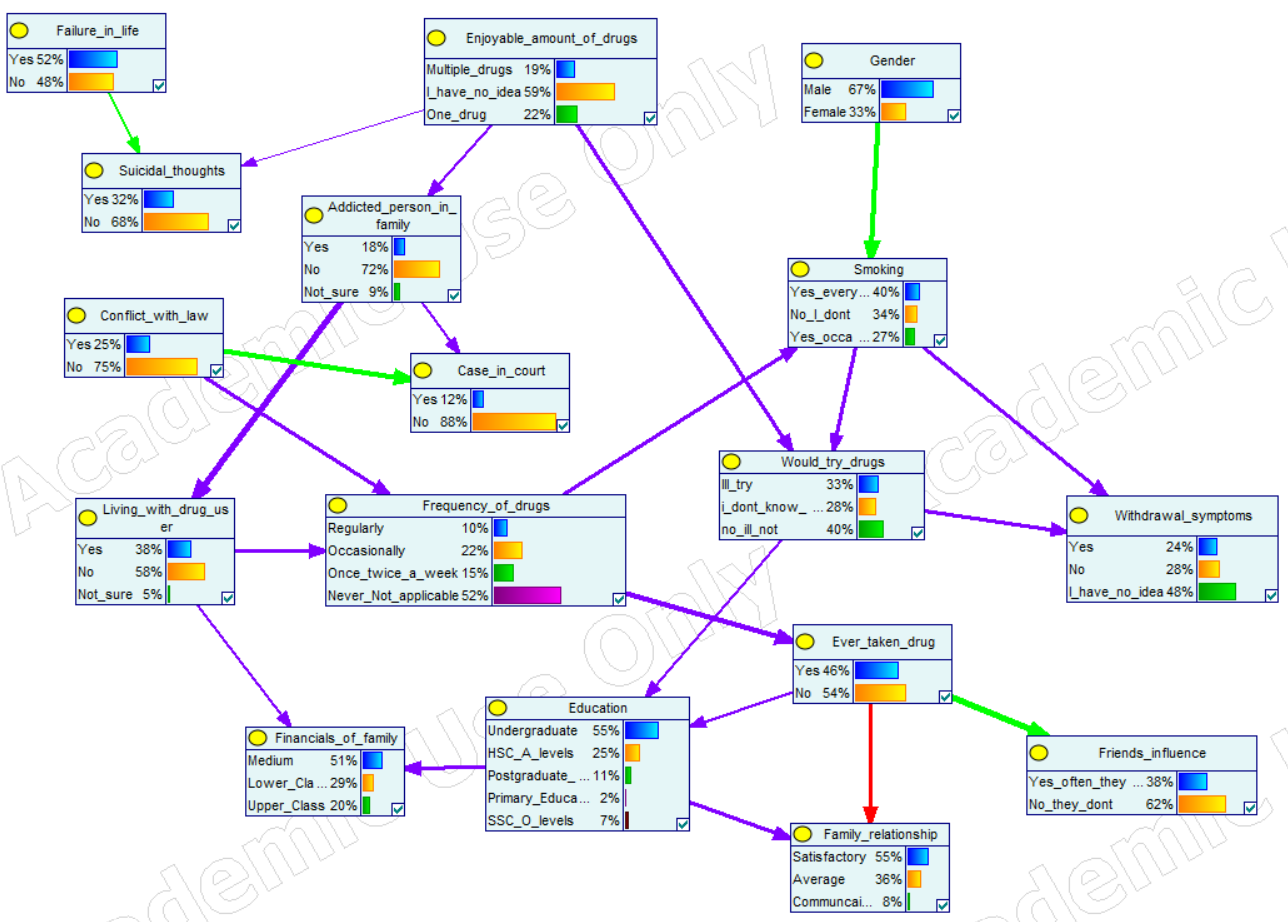
\includegraphics[width=\linewidth]{strengthinfluence/infleunce.png}
    \caption{Influence Relations in Bayesian Search Network.}
    \label{fig:influence_BN}
\end{figure}

\subsection{PC Bayesian Network}


\subsubsection{Accuracy}
The PC algorithm’s accuracy results are shown in Figure \ref{fig:PC_accuracy}. PC network achieved the highest accuracy while predicting the node.

\begin{figure}[h!]
    \centering
    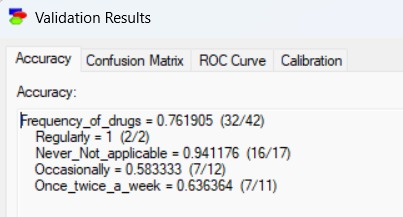
\includegraphics[width=\linewidth]{accuracies/PC_test.jpg}
    \caption{PC Network Accuracy of Prediction.}
    \label{fig:PC_accuracy}
\end{figure}

\subsubsection{Sensitivity Analysis}
In the PC network, the frequency of drug use is affected by age, amount of drugs, conflict with, living with a drug, user, and friends' influence as shown in Figure \ref{fig:sensitivity_PC}. This network represents a more nuanced outlook on factors affecting drug use than the Bayesian Search network. 

\begin{figure}[h!]
    \centering
    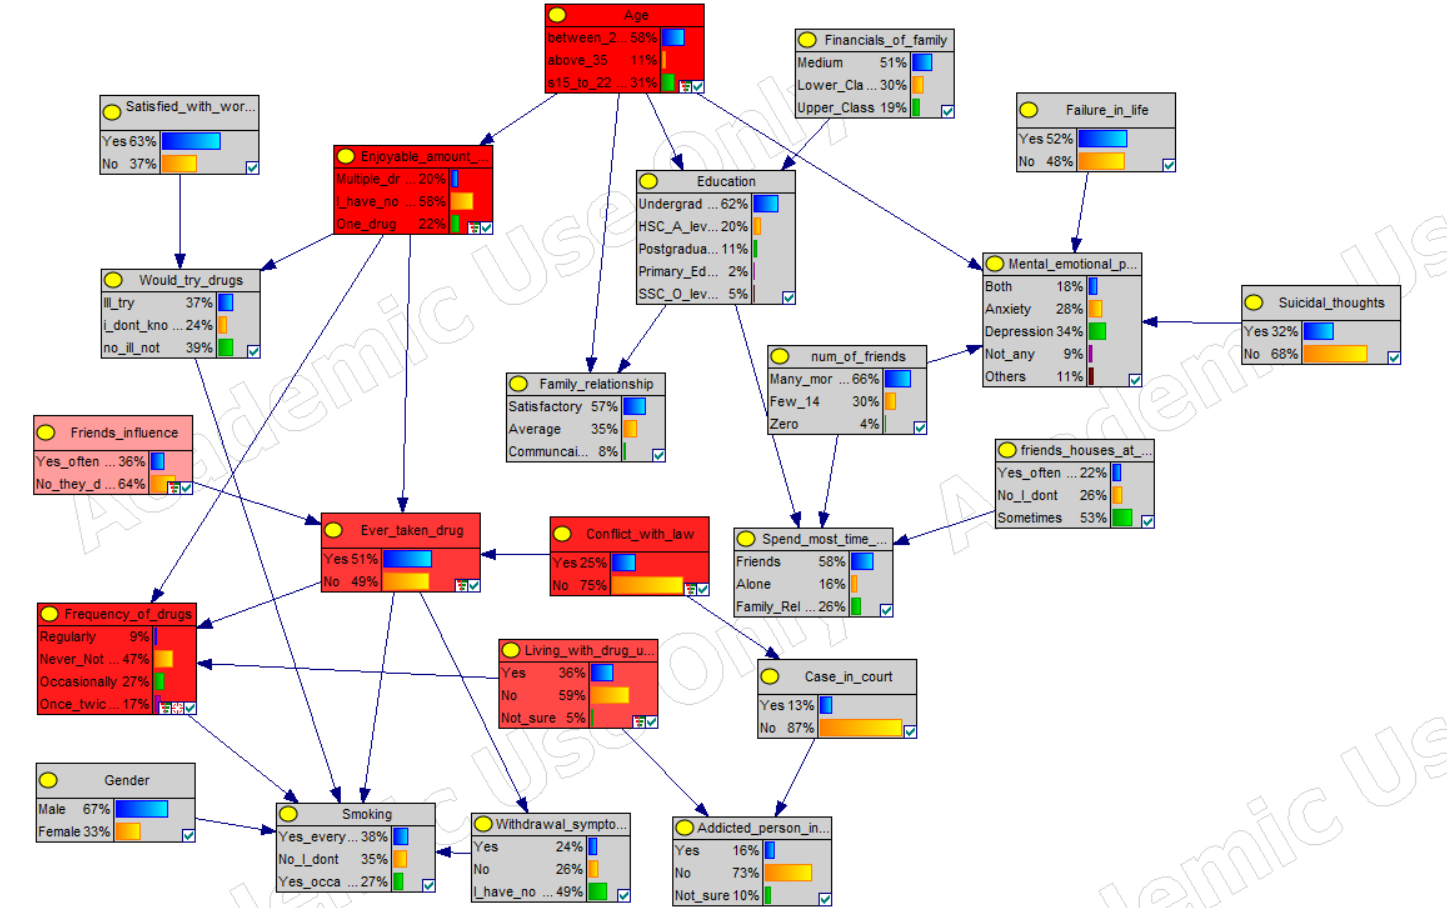
\includegraphics[width=\linewidth]{sensitivity/PC_sensitivity.png}
    \caption{Sensitivity Analysis of PC Network.}
    \label{fig:sensitivity_PC}
\end{figure}

\subsubsection{Influence Relations}
The influence diagram for the PC network contains the most number of ambiguous edges with only two clear positive influences. This could be the reason for the higher accuracy as the network might be fitting edge cases as well. The positive influences 
from conflict with law to case in court and living with drug user to addicted person in the family is consistent with the Bayesian Search network. However, here we have a positive influence going from case in court to addicted person in the family which is counter-intuitive. 


\begin{figure}[h!]
    \centering
    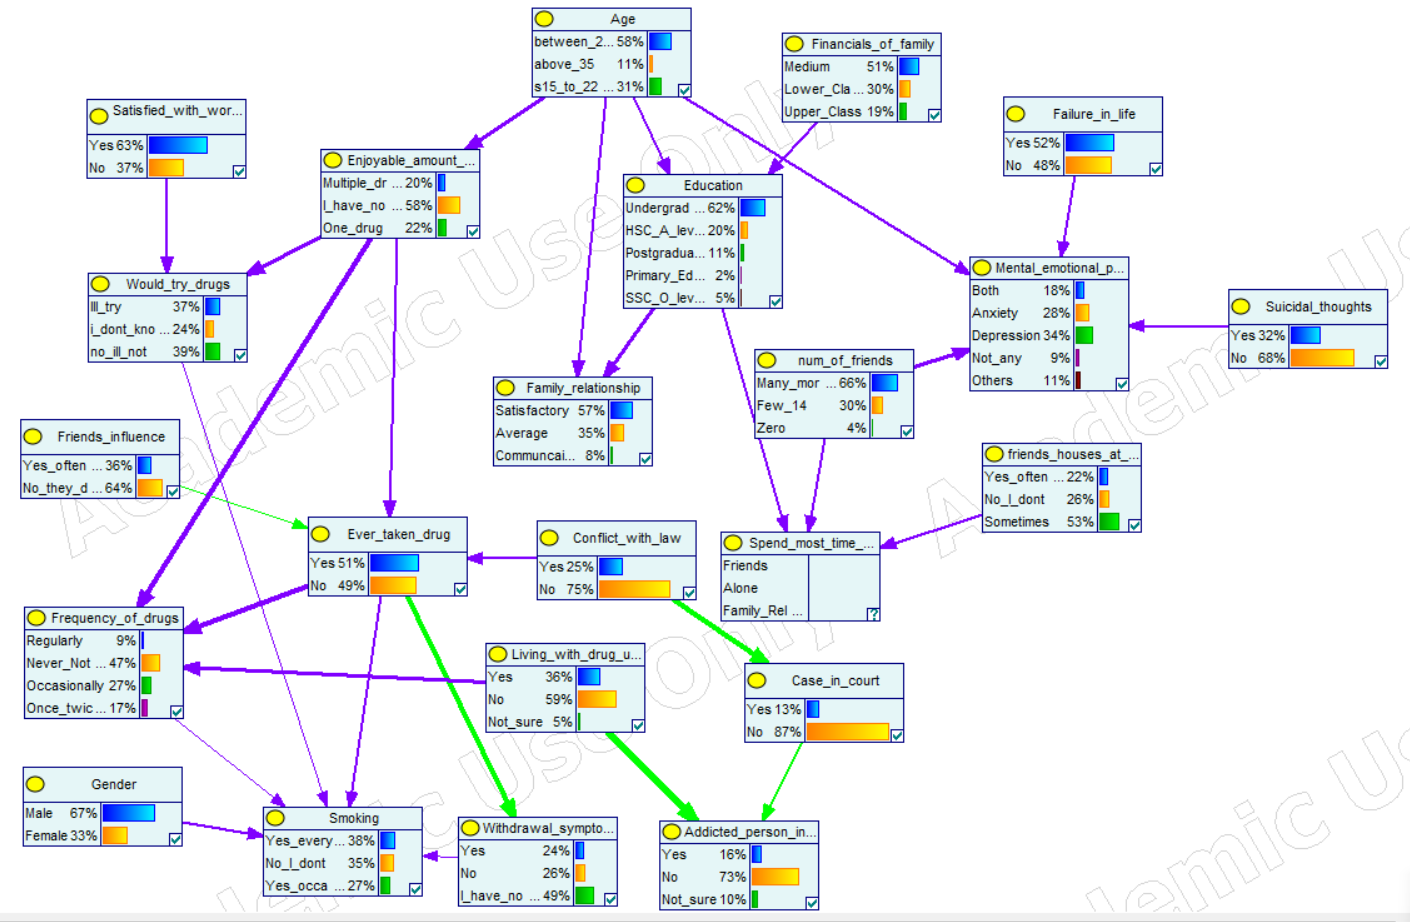
\includegraphics[width=\linewidth]{strengthinfluence/PC_influence.png}
    \caption{Influence Relations in PC Network.}
    \label{fig:influence_PC}
\end{figure}

\subsection{Greedy Thick-Thinning Bayesian Network}



\subsubsection{Accuracy}
The Greedy Thick-Thinning Bayesian network offers exactly the same testing accuracy for the frequency of drug use as well as shown in Figure \ref{fig:greedy_accuracy} 

\begin{figure}[h!]
    \centering
    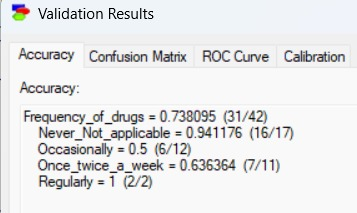
\includegraphics[width=\linewidth]{accuracies/greedy_testpng.jpg}
    \caption{Greedy Thick-Thinning Bayesian Network Accuracy of Prediction.}
    \label{fig:greedy_accuracy}
\end{figure}

\subsubsection{Sensitivity Analysis}
The sensitivity analysis for this Greedy ThickThinning BN as shown in Figure \ref{fig:sensitivity_greedy} indicates ever taken drug, enjoyable amount of drugs, and case in court to be the strongest factors for frequency of drug use. This BN also takes into account withdrawal symptoms, which is not done in any other BN we created. The strength of influence of conflict with law, however, is rather weak as compared to other networks. 

\begin{figure}[h!]
    \centering
    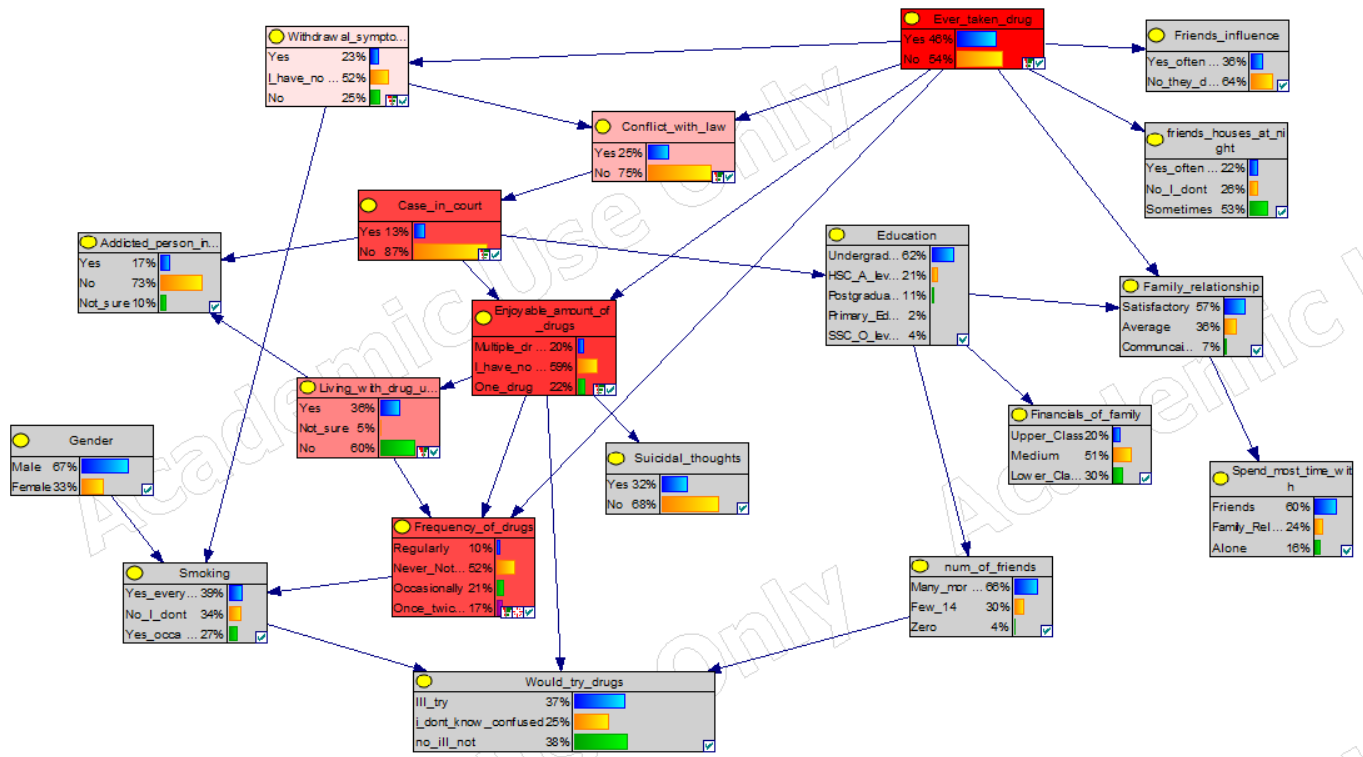
\includegraphics[width=\linewidth]{sensitivity/greedysensitivity.png}
    \caption{Sensitivity Analysis of Greedy Thick-Thinning Bayesian Network.}
    \label{fig:sensitivity_greedy}
\end{figure}

\subsubsection{Influence Relations}
The influence relations from the Greedy Thick-Thinning algorithm shown in Figure \ref{fig:influence_greedy} contains the most clear influences with positive influences. However, some edges such as ever taken drug to withdrawal symptoms, conflict with law, friends' influence, and friends house at parties are fairly counter-intuitive.

\begin{figure}[h!]
    \centering
    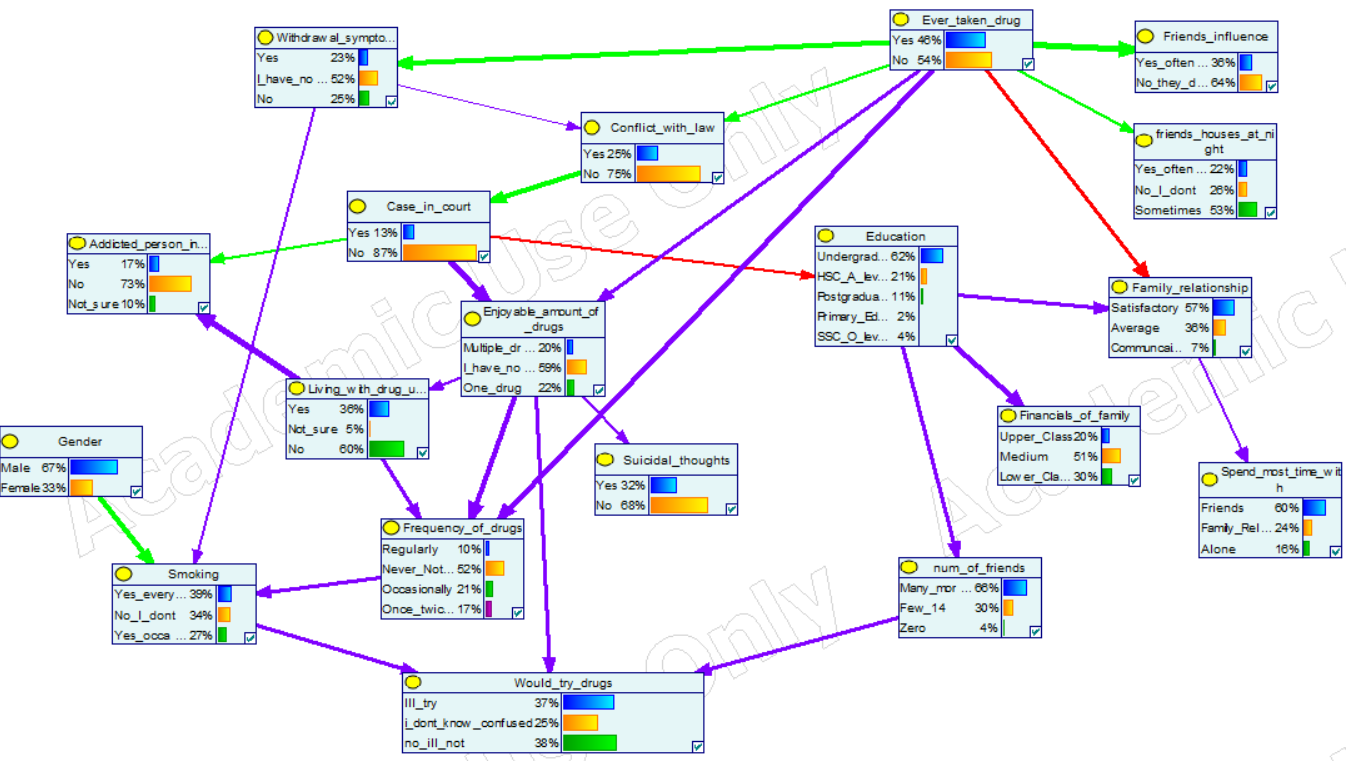
\includegraphics[width=\linewidth]{strengthinfluence/greedy_influence.png}
    \caption{Influence Relations in Greedy Thick-Thinning Network.}
    \label{fig:influence_greedy}
\end{figure}

\subsection{Algorithm Comparison}
We compared the three networks based on testing accuracy, training EM Log Likelihood, testing EM Log Likelihood, and Intuition. A comparison of the Bayesian Search, PC, and Greedy Thick-Thinning algorithms is summarized in Table \ref{tab:algorithm_comparison}. The testing accuracy was overall the same in all cases. However, the PC algorithm proved to be the highest in predicting the frequency of drug use nodes The EM Log Likelihood is almost the same for PC and Greedy Thick-Thinning algorithms, but the least is for the Bayesian Search network which indicates that it fits the data best among all. The EM Log Likelihood for testing accuracy is also calculated with Bayesian Search BN and Thick-Thinning algorithm indicating the same score, but PC BN has the lowest, favoring the fitness of the Bayesian Search again. 

\begin{table}[h!]
\centering
\caption{Comparison of Bayesian Search, PC, and Greedy Thick-Thinning Algorithms}
\label{tab:algorithm_comparison}
\renewcommand{\arraystretch}{1.3}
\resizebox{\columnwidth}{!}{%
\begin{tabular}{>{\raggedright\arraybackslash}p{5cm} >{\centering\arraybackslash}p{3cm} >{\centering\arraybackslash}p{3cm} >{\centering\arraybackslash}p{3cm}}
\toprule
\textbf{Metric / Parameter}       & \textbf{Bayesian Search}   & \textbf{PC Algorithm}   & \textbf{Greedy Thick-Thinning} \\
\midrule
\textbf{Best Training Accuracy}   & 0.751 (127/169)            & N/A                     & N/A                             \\
\textbf{Test Accuracy}            & 0.7381                     & 0.7619                  & 0.7381                          \\
\textbf{EM Log Likelihood}        & -3080.79                   & -3738.84                & -3660.4                         \\
\textbf{EM Log Likelihood Testing}    & -555.211                   & -687.617                & -555.631                         \\
\textbf{Score}                    & N/A                        & -4308.85                & N/A                             \\
\textbf{Elapsed Time (s)}         & 0.937                      & 0.078                   & 0.063                           \\
\textbf{Iterations}               & 100                        & N/A                     & N/A                             \\
\textbf{Algorithm Type}           & Score-Based                & Constraint-Based        & Score-Based                     \\
\textbf{Background Knowledge}     & Forbidden Arcs: 49         & Forbidden Arcs: 49      & Forbidden Arcs: 49              \\
\textbf{Max Parent Count}         & 4                          & 4                       & 4                               \\
\textbf{Intuition}                & Most Intuitive             & Fairly Intuitive        & Least Intuitive                               \\
\bottomrule
\end{tabular}%
}
\end{table}
The Bayesian Search Algorithm achieved a testing accuracy of 73.81\%, demonstrating a reasonable consistency in predictions without overfitting the data. This structure had the smallest number of direct influences on the target node with just "Conflict with law" and "Living with drug user" having edges to "Frequency of drugs." While it did have some counter-intuitive relationships between variables such as "Enjoyable amount of drugs" impacting "Would try drugs" and "Ever taken drug" to "Friends influence", for the most part, it logically resulted in the best structure that closely resembled real world dynamics. However, with a runtime of 0.937 it was the slowest of all the algorithms.

The PC Algorithm demonstrated the highest testing accuracy of 76.19\%, making it the most accurate of the three models for predicting drug use frequency. By using rigorous statistical methods, it eliminated weaker connections but was still dominated by ambiguous relationships and counter-intuitive relationships such as "Age" impacting "Enjoyable amount of drugs", "Case in court" to "Addicted person in the family", "Suicidal thoughts" to "Mental emotional problems" along with many others. It was computationally effective with a time of 0.078 seconds.

The Greedy Thick-Thinning Algorithm matched the testing accuracy of the Bayesian Search Algorithm at  73.81\%, but it completed its run in 0.063 seconds making it the fastest of the three. Its sensitivity analysis revealed that it found the least amount of ambiguous influence between nodes of the three models indicating that it produces a clearer and more decisive representation of the relationships among variables however this can also imply that the algorithm sacrifices some of the nuanced, indirect relationships captured by the other models, potentially leading to an oversimplified representation of complex dependencies.

\section{Conclusion}
Our networks prove that socioeconomic factors and demographics play a significant role in determining the likelihood of individuals' increased intake of drugs. Our networks also validate the common gendered perspectives in South Asian society where men are more socially accepted smokers. Our likelihood P(Smoking | Male) = 88.88\% is consistent with this practice. However, gender appears to have less of impact of the frequency of drug usage, further supporting the claim that the issue goes beyond gender with drug usage being on the rise in females too. 

Perhaps the most concerning fact that we seem to have uncovered is that individuals with regular drug usage being more likely to have suicidal thoughts. The initial probability of having suicidal thoughts is said to be 32\% in the dataset but it jumps to 50\% for frequent drug users.

Conflict with the judicial system appears to influence individuals' drug consumption practices across all three networks, while those living with drug users are more likely to have increased intake. Smoking is a significant indicator of susceptibility to drug addiction and the subsequent occurrence of withdrawal symptoms. Friends' influence and educational level have also been identified as contributing factors to the culture of drug usage. Overall, conflict with the law and living with drug users emerged as the leading factors in our sensitivity analysis. This suggests that susceptibility to heightened drug use, and potentially addiction, stems from a history of criminal involvement and exposure to drug use.

\section{Future work}
In terms of research, additional work in the field needs to be done, collection of larger datasets to reduce bias and improve generalization, especially to the under-represented groups such as women for whom drug use has been on a steady rise. The collection of more data would also allow for further nuance through the addition of variables such as mental health history, peer pressure intensity, or socioeconomic stressors for gaining a deeper insight into latent factors influencing drug addiction.

From an administrative standpoint- Bangladesh needs a shift towards evidence-based policies and strategies that prioritize prevention, harm reduction, and intervention programs over punitive measures to better tackle the root causes of drug abuse. Work needs to be done in terms of developing more effective and accessible rehabilitation facilities, particularly in high-risk zones where drug usage is most prevalent. These programs should focus on mental, and emotional health as well as physical health. Better measures need to be taken to increase public awareness about drug addiction, its risks, and available treatments while combating the stigma associated with seeking help that exists due to the illegal status of drug use within The development of confidential and secure channels for individuals to reach out without fear of legal repercussions is vital.

With the model, there remains scope for improvement with further fine-tuning of relationships with additional data or additional training iterations, as well as further exploration of alternative structure learning algorithms to further optimize the predictive performance beyond the current 70\% accuracy. Work could also be done to extend the current Bayesian Network into a Dynamic Bayesian Network (DBN) to account for temporal changes in drug usage behavior over time enabling the tracking of individuals’ progress or regression in drug addiction.

% The preferred spelling of the word ``acknowledgment'' in America is without 
% an ``e'' after the ``g''. Avoid the stilted expression ``one of us (R. B. 
% G.) thanks $\ldots$''. Instead, try ``R. B. G. thanks$\ldots$''. Put sponsor 
% acknowledgments in the unnumbered footnote on the first page.

\bibliographystyle{IEEEtran}
\bibliography{references.bib}

% \vspace{12pt}
% \color{red}
% IEEE conference templates contain guidance text for composing and formatting conference papers. Please ensure that all template text is removed from your conferencbeforeprior to submission to the conference. Failure to remove the template text from your paper may result in your paper not being published.

\end{document}
